\subsection{Run 3 Simulation Strategy}
Monte Carlo simulations account for more than 60\% of the CPU hours consumed by the ATLAS experiment, as shown in Figure \ref{fig:Run3CPUbyActivity} for Run 3. At the same time the physics reach of many analyses, including precision measurements in the Higgs sector is limited by the available statistics of MC events. Reducing the amount of time spent on simulations is a priority  for the HL-LHC R\&D program. This problem is being tackled on many fronts by ATLAS, by the G\textsc{eant}4 collaboration, and by multiple R \& D projects aimed at developing accelerator-friendly detector simulation tools.

\begin{figure}
    \centering
    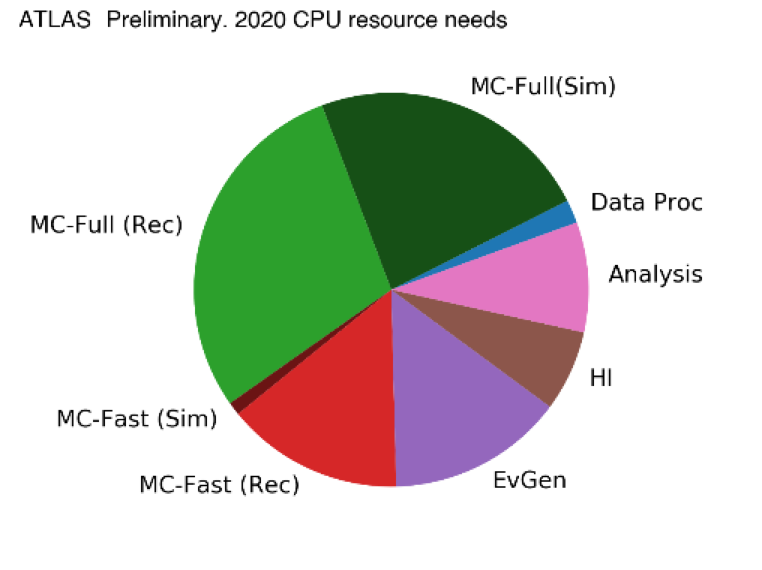
\includegraphics[width=0.70\textwidth]{figures/ATLASpreliminary2020CPUResourceNeeds.png}
    \caption{ATLAS CPU hours budgeted for various activities in 2020}
    \label{fig:Run3CPUbyActivity}
\end{figure}


ATLAS currently uses both Full simulation (FullSim based on G\textsc{eant}4) and Fast simulation (primarily parametrized calorimeter response) for physics results. Each physics analysis group evaluates the requirements for statistical and systematic precision for each physics sample that needs to be simulated. Based on these studies, physicists request some simulation samples with higher precision FullSim, and others with lower precision fast simulation. Reconstruction time for simulated events are currently similar for both simulation methods (but see FastChain discussion in next section). On average, currently about 50\% of all samples use FullSim. For the HL-LHC we aim to reduce this fraction to 25\%, thereby saving half of the CPU resources devoted to detector simulation at the HL-LHC. 

Besides reducing the fraction of events simulated with G\textsc{eant}4, we have an active R\&D program aimed at optimizing the CPU requirements of G\textsc{eant}4. Performance gains of ~20\% with no impact on physics performance have been already demonstrated and another ~20\% should be achievable.  The FullSim configuration for Run 3 will include the use of "Frozen Showers" in the forward region as in Run 1 and Run 2.

Reducing the fraction of MC simulated using FullSim requires analysers to be confident in using samples produced using fast simulation techniques in their analyses.  The agreement between full and fast simulation (and data) for key features of physics distributions has to be good enough that analyses are not biased.  In ATLAS this is mostly determined by the Combined Performance (CP) Groups who are responsible for producing the calibrations which allow comparison between data and MC.  The goal for Run 3 is for FullSim and fast simulation to agree to within uncertainties in the CP Group calibrations, so that the same calibrations can be used for all MC samples.  CP Group calibrations take a lot of person-hours to produce, so there would be reluctance to introduce an extra set of calibrations.

It should be noted that despite the goal of reducing the fraction of events simulated using G\textsc{eant}4 in Run 3, G\textsc{eant}4 will remain a critical part of our simulation strategy. It will be used to produce the samples used to tune parameterizations used by the fast simulation and will continued to be developed to give an improved description of interactions in the detector. A key improvement planned for Run 3 is to include energy deposits made directly by B's, D's and $\tau$ leptons, which in Run 2 were dealt with solely by the Generation step. This blurring of the line between Generation and Simulation will continue in Run 3 as G\textsc{eant}4 works to include b-physics in their physics lists.

For Run 3 ATLAS will combine hard-scatter and pile-up events at the digit (RDO) level.  The approach will be to make pre-mixed pile-up datasets by combining minbias events simulated by Geant4 and digitizing them together in the absence of a hard-scatter event. The pre-mixed pile-up RDO datasets will then be stored on the grid.  In the main production workflow hard-scatter events will be digitized then "overlaid" on top of a pre-mixed pile-up RDO event.  This process is considerably (quantify) faster than, and with much reduced I/O requirements compared to, pile-up digitization and scales much less steeply with pile-up luminosity.  As long as each pre-mixed pile-up RDO event can be used more than once then there is a reduction in resource requirements.  A strategy for how best to store and access the O(PB) pre-mixed RDO datasets will be developed over the next few months.  Another new issue for Run 3 is the variation of the beamspot size at the same time as $\langle\mu\rangle$ is varying.  The simplest way to deal with this is to have multiple (three?) sub-campaigns for each data period each simulated with a different beam spot width.  All but the last sub-campaign will look at beam conditions during the luminosity levelling regime, so $\langle\mu\rangle$ will be constant. The final sub-campaign will replicate the beam after levelling has finished and so will have a variable $\langle\mu\rangle$ value.
%\begin{itemize}
%    \item (shower libraries dead after Run 3)
%    \item implications on computing model.
%\end{itemize}
\subsection{Run 4 Strategy}
Run 4 analyses will need ten times more MC events than previous campaigns, so O(200) billion events. It will not be possible to produce this much MC using FullSim or even with Fast Simulation. For Run 4 ATLAS will need to switch to FastChain as the baseline simulation approach. For the simulation step, this involves using an ACTS-based fast Track simulation for the Inner Detector and FastCaloSim for the Calorimeter. Doing this will make the simulation time small compared to the reconstruction time, so further speed-ups to the MC production workflow will require reducing the reconstruction time (Add reference).  One possible idea is to use Trigger-like Algorithms to filter events prior to reconstruction, so that events which will never be used in analyses are not reconstructed (or written out). Another idea would be to use a strategy like Overlay, but to reconstruct the pile-up tracks in separate job, producing RDO-prime files containing pile-up tracks. These tracks could be copied through the overlay step. Reconstruction would then consist of running tracking for the hard-scatter, then combining the track collections and using the merged track collection as the input to the rest of the reconstruction.
Even if it is possible in principle produce the required sample sizes, they will still need to be stored somewhere. Current projections suggest that it will not be possible to store the required samples on disk.  Not storing intermediate file formats is a possible way to reduce the disk requirements.

\subsection{R \& D needed for Run 4} 
\begin{table}[htb!]
  \caption{Monte Carlo Chain CPU times in HS06~$\times$~seconds. Full Sim is Geant4+Frozen Showers in the FCAL. Fast Simulation is FastCaloSim V2 in the Calorimeter and G4 elsewhere. Full digi is digitizing hard-scatter and minbias hits together.
  MC Overlay is digitizing the hard-scatter and then combining with a pre-digitized zerobias event. Fast Chain is simulation using FATRAS in the Inner Detector, FastCaloSim V2 in the Calorimeter and Geant4 in the Muon System; digitizing the hard-scatter and combining with a pre-digitized zerobias event, where ID Tracking has already been performed. Standard reconstruction is assumed, except for the Fast Chain case, where ID Tracking is performed for the hard-scatter only.}
  \label{tab:SimCPU}
  \centering
  \begin{tabular}{|c||c|c|c||c||c|} \hline
    scenario & Hard-scatter & Hard-scatter & Hard-scatter & Background & Hard-scatter \\
             & EVNTtoHITS & HITStoRDO & RDOtoESD & from table 2 & Total \\ \hline
    Full sim $+$ & 5684 & $\langle\mu\rangle=$140: 3317         & 402        & 23 & 9403 \\
    Full digi &   & $\langle\mu\rangle=$200: 4233         & 584        & 33 & 10534 \\   
    Full sim + & 5684 & $\langle\mu\rangle=$140: 183          & 402        & 92 & 6351 \\
    MC Overlay &   & $\langle\mu\rangle=$200: 202 & 584        & 121 & 6611 \\   
    Fast sim + & 1137 & $\langle\mu\rangle=$140: 183          & 402        & 92 & 1814 \\
    MC Overlay &   & $\langle\mu\rangle=$200: 202 & 584        & 121 & 2044 \\
    Fast Chain + & 114 & $\langle\mu\rangle=$140: 183          & 278        & 95 & 669 \\
    MC Overlay &   & $\langle\mu\rangle=$200: 202 & 370        & 126 & 811 \\ \hline
    \end{tabular}
    % Sim + Digi numbers taken from results of running in 21.9 provided by Markus
    % Reco numbers taken from table in section 6.5
    % Newer G4 version will be faster
    % Assuming MC Overlay time is negligible (need a better estimate).
    % From the Overlay note: For the standard method, at μ=70 the CPU time required is 7.5 times larger than for μ=10. For the MC-overlay method the increase in CPU time is only 20% when increasing μ from 10 to 70. Extrapolating this to μ=200 the CPU time is 20 times higher for the standard method and < 2 times higher for the MC-overlay method.
    % Assuming G4+FCS is 5 times faster than full G4
    % Assuming that FATRAS (ID) + FCS + G4 (MS) is 10 times faster than G4+FCS
    % Assuming that running ID Tracking on zero bias will make reco tracking time negligible (probably wrong)
\end{table}

\begin{table}[htb!]
  \caption{Monte Carlo Background costs per hard-scatter in HS06~$\times$~seconds. Re-use factors are the number of times these events are re-used later in the workflow. The assumption here is that the size of the minbias HITS and zerobias RDO samples will scale with $\langle\mu\rangle$ }
  \label{tab:SimCPU}
  \centering
  \begin{tabular}{|c||c|c|c|c|c|} \hline
             &  Production & Re-use & $\langle\mu\rangle$ & No. used per & Cost per \\ 
             &  [HS06s] & factor & & Hard-scatter & Hard-scatter [HS06s]\\ \hline
    Low pT minbias & 2120 & 1867200 & 140 & 5446 & 6\\
    Low pT minbias & 2120 & 1867200 & 200 & 7780 & 9\\
    High pT minbias & 5787 & 4800 & 140 & 14 &  17 \\
    High pT minbias & 5787 & 4800 & 200 & 20 &  24 \\
    Zerobias RDOs & 3317 & 48 & 140 & 1 & 69 \\
    Zerobias RDOs & 4233 & 48 & 200 & 1 & 88 \\
    Zerobias RDOs + ID Tracks & 3441 & 48 & 140 & 1 & 72 \\
    Zerobias RDOs + ID Tracks & 4447 & 48 & 200 & 1 & 93 \\ \hline
    \end{tabular}
  

    % Sim + Digi numbers taken from results of running in 21.9 provided by Markus
    % Reco numbers taken from table in section 6.5
    % Newer G4 version will be faster
    % Assuming MC Overlay time is negligible (need a better estimate)
    % Assuming G4+FCS is 8.5 times faster than full G4
    % Assuming that FATRAS (ID) + FCS + G4 (MS) is 10 times faster than G4+FCS
    % Assuming that running ID Tracking on zero bias will make reco tracking time negligible (probably wrong)
\end{table}
%\begin{itemize}
%    \item Justify sample sizes required (disk requirements)
%    \item Nature of the samples: CP samples, background samples.
%    \item {\it \color{blue}  Number of fast simulation flavours: multiple flavours require %multiple validations/calibrations. OTH multiple flavours can be optimized for different analyses.
%    \item Run 4 baseline: FastChain}
%\end{itemize}
Detector simulation is projected to continue to be one of the main consumers of CPU resources in Run 4 and beyond. ATLAS is eager to collaborate with international efforts to parallelize G\textsc{eant}4 detector simulation. Preliminary evaluations and prototyping in the areas of G\textsc{eant}4 EM physics and particle transport indicate that a substantial speedup in G\textsc{eant}4 event throughput is possible on a time scale of 5-10 years.

Development will be required to produce MC Overlay events at $<\mu>=200$. MC Overlay events are currently produced using the pile-up digitization workflow used in Run 2. This approach is not compatible with AthenaMT running. Most likely this approach will be used for Run 3, but it will not be suitable for the high $<\mu>$ values expected in Run 4. This will involve sharing background minbias events between multiple threads.

Finally a rich ATLAS-wide R\&D program in collaboration with others is aimed at developing fast, high-fidelity detector simulation using generative neural network models. Depending on the fidelity achieved by these models in simulating tails in the detector response, another factor ~2x may be saved in CPU resources for simulation by producing fewer events simulated with full G\textsc{eant}4.





%\begin{itemize}
%    \item Strategy to store O(200B) MC events, 
%    \item Continue investigating role of GANs. Discuss training samples size.
%    \item External R\&D needed: parallelising Generators and Geant4
%\end{itemize}
\subsection{Discussion on number of events needed}

\subsection{Trigger simulation}
The Run~4 trigger system consists of a hardware and software trigger system~\cite{ATLAS-TDR-29}. The hardware trigger is simulated using dedicated algorithms that strive to perform a bit-wise correct emulation of the trigger decision. The majority of the system consists of FPGA-based electronics that can be simulated on a regular CPU without much performance penalty.

The Hardware Track Trigger (HTT) on the other hand uses a custom associative memory chip to perform massively parallel pattern look-ups for finding track candidates.
Regular ATLAS simulation and reconstruction will use the parameterised fast simulation (FastHTTSim), which applies smearing of offline/truth/HLT track parameters, with negligible need of resources. 
The resource intensive full HTT simulation (HTTSim), will only be used for the following use-cases: performance studies at high pile-up in a limited $\phi$ slice (1/32); estimation of fake and dataflow rates with high-pileup samples; parameterisation of the fast simulation using single-muon events. The generation of constants for the pattern-matching and track-fitting (HTTSimGen) requires high statistics samples of simulated single-muon events. 

The required CPU resources for one production cycle are summarised in Table~\ref{tab:httsim}. A new production will be required when data-taking conditions (e.g. tracker alignment, LHC interaction region) change significantly and is estimated to about two cycles per year. Additional cycles will be needed during the commissioning phase of the project. HTT validation may also need additional samples to study tracking performance in dense environments.

The samples sizes and event processing times are conservative estimates with very large uncertainties derived from previous FTK studies. Further detailed studies are needed to get better estimates on samples sizes and processing times. To reduce the required resources, alternative processing methods are under consideration, like the usage of GPUs or the possibility to process simulated data directly on the HTT hardware system at Point-1. 

\begin{table}[h]
    \centering
    \begin{tabular}{|l|l|l|r|r|r|}
      \hline
      use case                  & sim. type &  event type & events/cycle & HS06/event & HS06/cycle \\
      \hline
      ATLAS simulation          & FastHTTSim  & any         &  any   & negligible & neglible \\
      Performance high-PU       & HTTSim  & min-bias   & 1 M  & 1.2 M/32 & 37500 M\\
      Fake and dataflow  high-PU & HTTSim  & min-bias   & 50 k   & 1.2 M & 60000 M\\
      Parameterization          & HTTSim  & single muons    & 50 M   & 100 & 5000 M\\
      Generation of constants  & HTTSimGen & single muons   & 1 B   & 135 & 135000 M\\
    
      \hline
    \end{tabular}
   \caption{Extrapolations of CPU resources for global HTT during regular data-taking per production cycle (see text). A CPU reduction of 20\% per event is expected if only regional HTT is simulated.}
    \label{tab:httsim}
\end{table}

%\subsection{Impact}
%The results of these R\&D efforts will have a 2-16X impact on the resources needed for MC simulations at the HL-LHC, as described in this document.
